\chapter{Introduction}
\addtitlethumb{Frontmatter}{\huge 1}{white}{gray}


\section{Introduction}\label{sec:intro_intro}

For almost a century, computational machines have been used as a tool to improve scientific research. In part driven by national security concerns during the First and Second World Wars as well as the Cold War, increasingly complex computers have been designed. Early computers were entirely designed for application-specific tasks, with a large drive behind them being nuclear simulations for the Manhattan project. In 1945, the popular Von-Neumann architecture was developed with the goal of making Monte Carlo simulations easier to develop and to facilitate general purpose computing. This architecture was a significant improvement over previous computers where changing the program required physically flipping switches and changing cables on the computer itself. One of the first computers built according to the von-Neumann architecture was the MANIAC computer commissioned by Los Alamos National Laboratory, seen on the left in Figure \ref{fig:intro_supercomputers}.

With the advancement of an architecture that treats code and data identically, it was possible to create more complex programs including compilers: programs that could create machine code from human-readable code. As the 50s and 60s passed, general purpose computers were increasingly used in science. From weather dynamics to fluid dynamics, from chaos theory to game theory, these computers were being adopted by a wide range of scientific fields. Astronomy was likewise also a driving force for computational innovation. In 1953, for example, the first high-level programming language for IBM computers was developed by John Backus, a programmer frustrated with the difficulty of accurately calculating the moon's position using only machine code. John Backus' `Speedcode' was a direct predecessor of Fortran, a language developed at IBM in the '50s and still used by the scientific community today. Another important discovery on our road was the Fast Fourier Transform (FFT), discovered by two researchers from Princeton and IBM. The FFT has been described as `the most important numerical algorithm of our lifetime' and the author's personal favourite `an algorithm the whole family can use'\citep{top_10_algos}. As we will soon see, Radio Astronomers quickly became part of this family.

\begin{figure}[h]
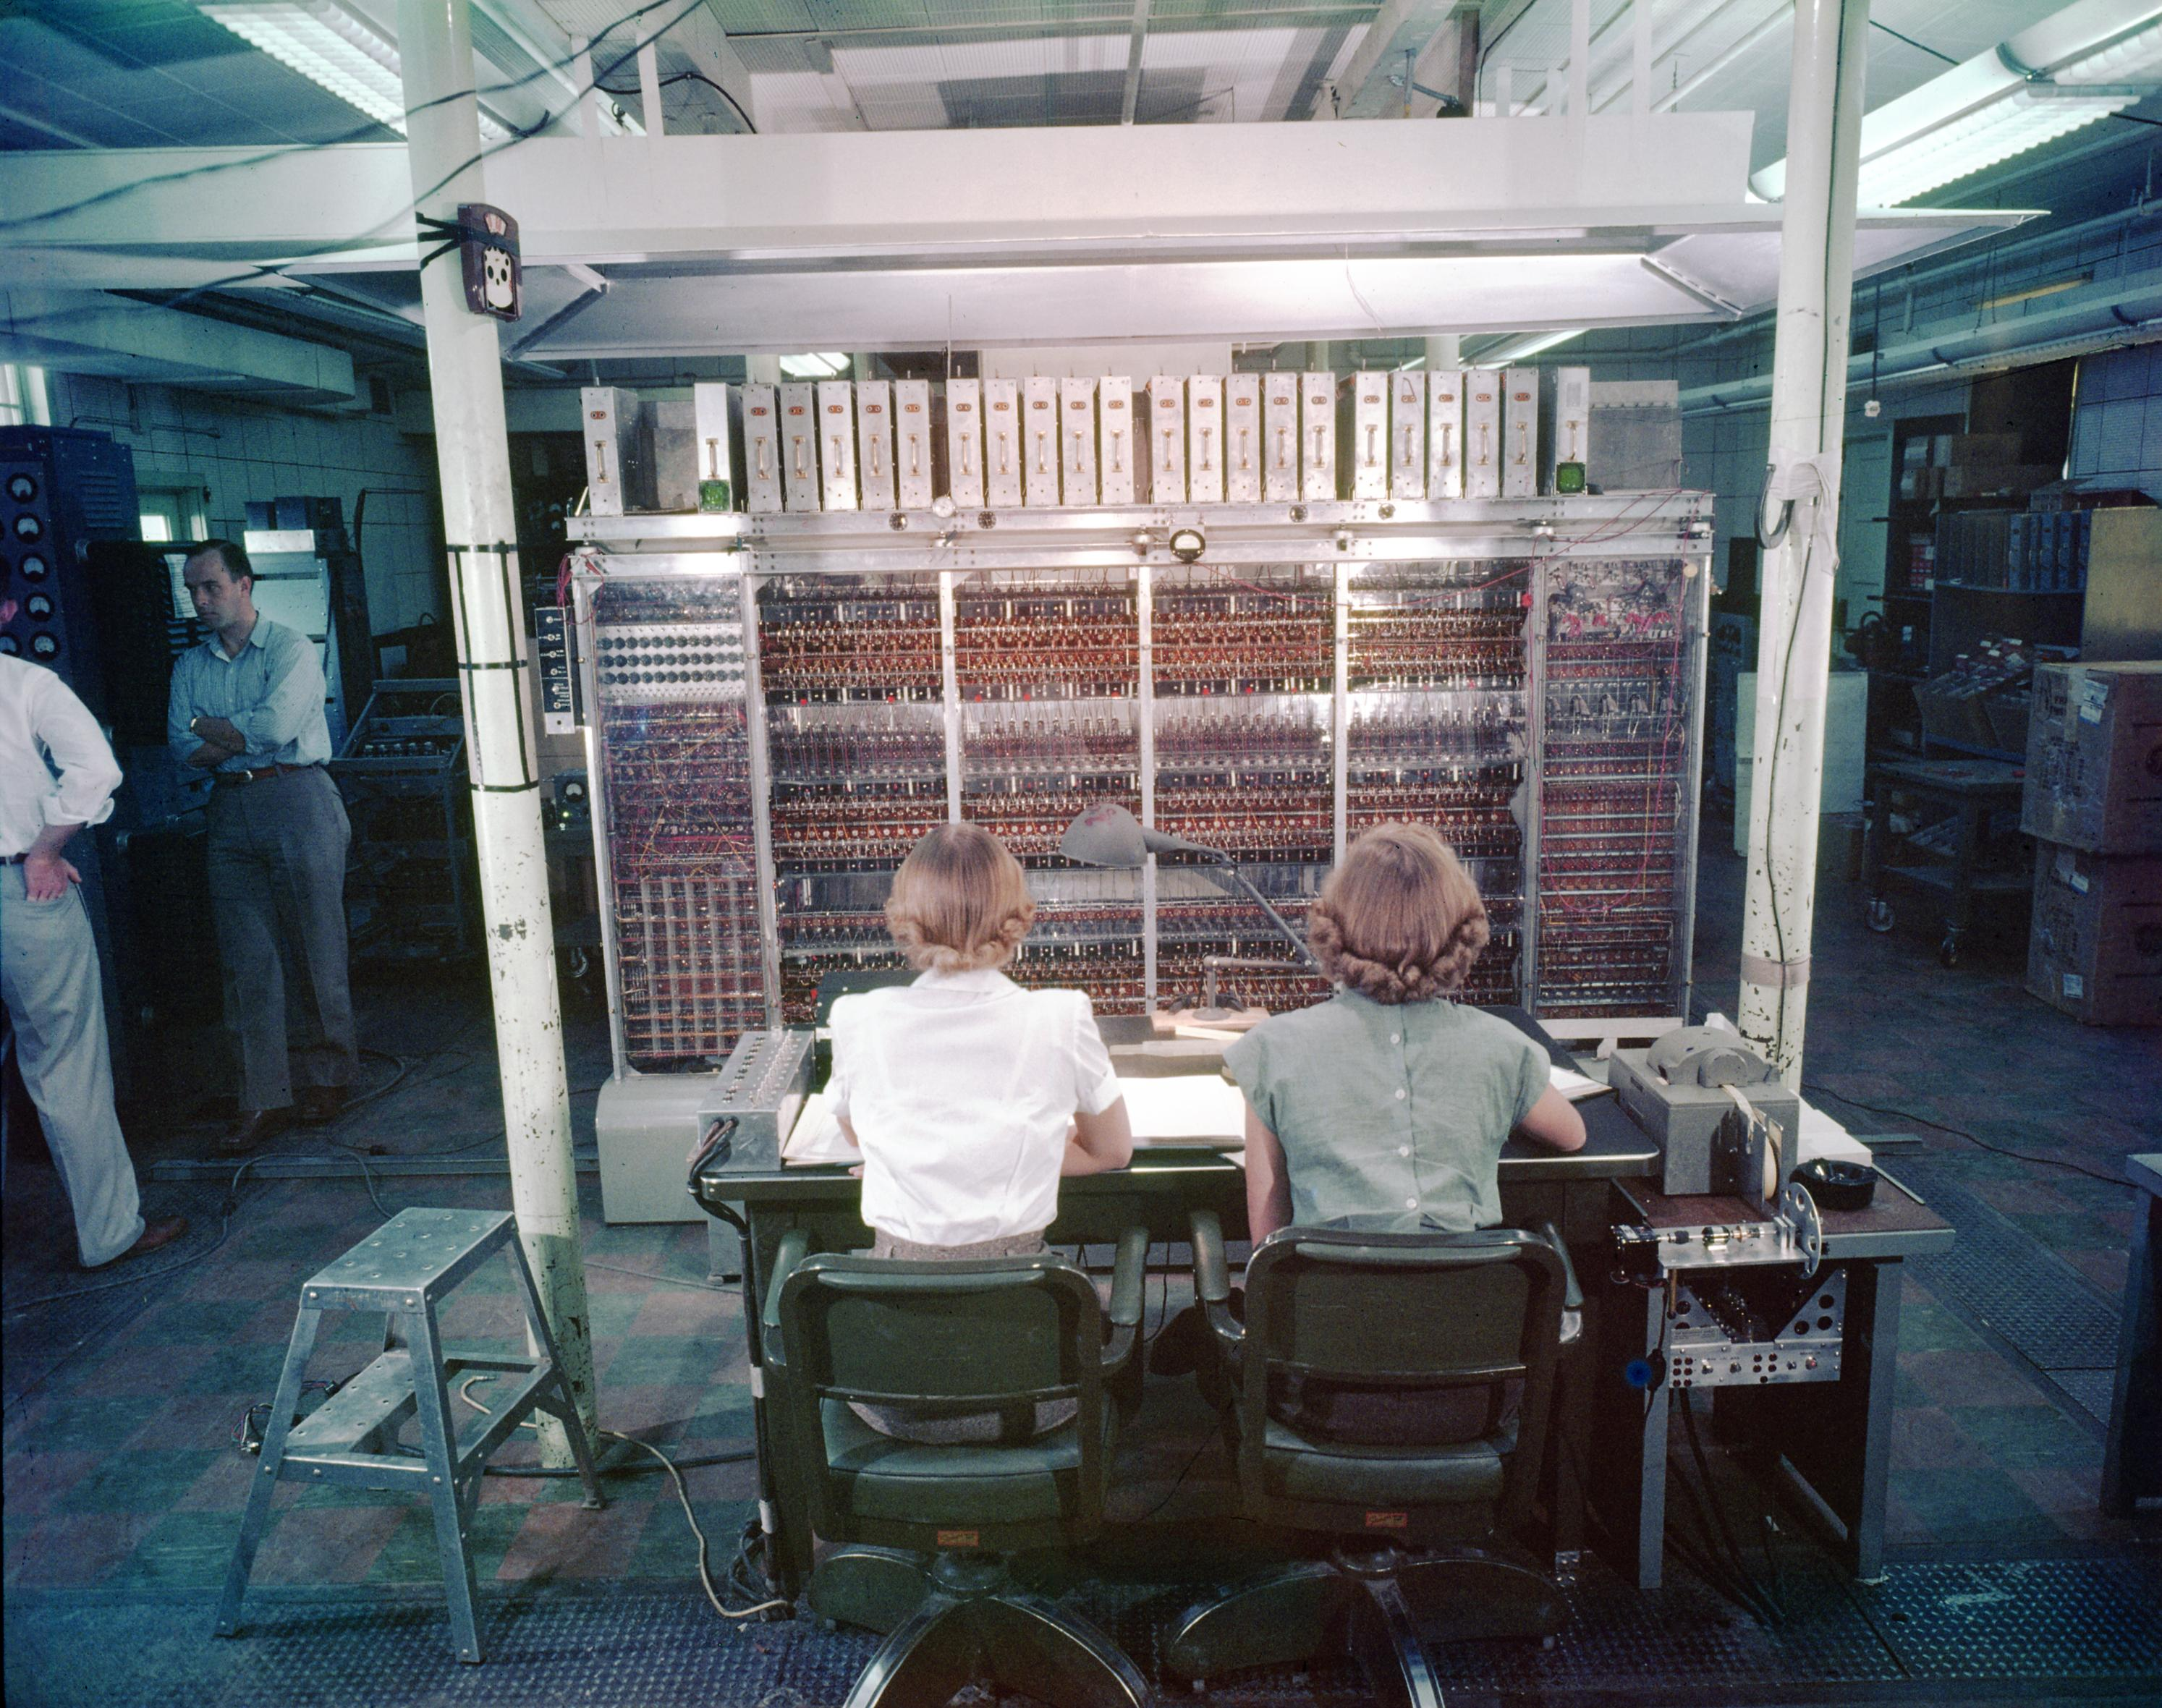
\includegraphics[width=.45\linewidth]{background/figures/Maniac_1952.jpg}\quad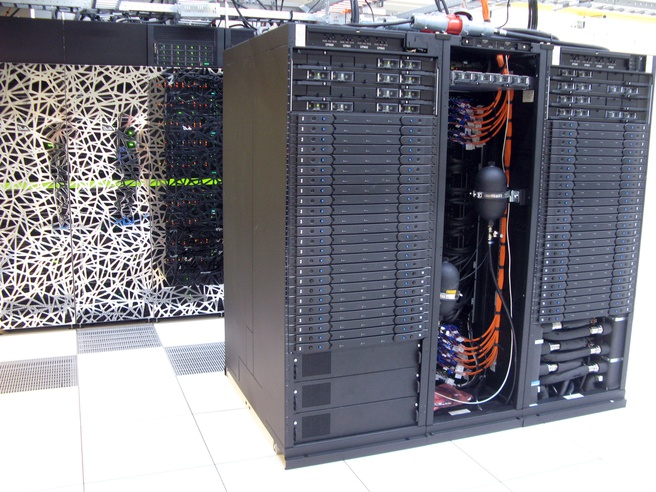
\includegraphics[width=.45\linewidth]{background/figures/cartesius.jpeg}
    \caption[Two supercomputers sixty years apart.]{Two supercomputers sixty years apart. On the left is the MANIAC computer from 1952 at Los Alamos, while on the right is the Cartesius cluster at SURFsara, Amsterdam in 2018.}
    \label{fig:intro_supercomputers}

\end{figure}

As computers became more available, they were increasingly adopted by universities and research institutes. In the '70s, computers began to talk to each other over a network connection. This capability not only made scientific collaboration easier but made it possible to distribute computation across multiple sites. Moreover, the development of the integrated circuit and subsequent drop in price/performance of computers made it financially feasible for scientific institutes to purchase multiple computers dedicated to scientific research. As hardware, networks, and software matured, computer clusters became more widely used\citep{tel_2000}. In part because of their cost effectiveness, and potential for parallelization, clusters of computers became more widely used as the 80's wound down. By then, general purpose computing was widely adopted by the astronomical community. By then several astronomical software suites have been developed, with software such as AIPS and IRAF and standards such as FITS used to this day. 

The '90s continued the distributed computing trend with the appearance of commodity compute clusters, with virtual `supercomputers' being created from Commercial Off-The-Shelf (COTS) hardware, and networking. These clusters became quickly adopted by scientists to perform simulations and data processing. Around the same time, the idea of 'grids' was created. The concept was that of a country, continent or even world-wide network of hardware that can transparently handle distributed tasks, and provide researchers with a vast pool of resources. Grid processing was pioneered by CERN with the goal of meeting the computational and storage requirements of their High Energy Physics modelling and data reduction. While this infrastructure was originally built for HEP experiments, it is also useful for other scientific projects, particularly low-frequency Radio Astronomy. 


\subsection{Astronomy and Computing}

Since the early days of computing, the field of astronomy has embraced digitization of data acquisition and processing. Being able to store astronomical data digitally makes it possible to transfer, copy, backup and process them easily. With the rapid development of CCDs, optical astronomy entered the digital age, however with the wide availability of Analog-Digital Converters (ADCs), radio astronomy has been digital since the 1970s. By the end of the '70s, the Very Large Array (VLA) in New Mexico and the Westerbork Synthesis Radio Telescope (WSRT) had consistently been using processing pipelines with imaging algorithms taking advantage of the FFT developed a decade earlier\citep{clark1980_clean}, running on Digital Equipment Corporation's line of PDP, and later VAX, minicomputers. 

With the complete digitization of astronomical observations, over the past decade,  all of astronomy has entered the big data regime. As of 2019, there are multiple planned and ongoing large-scale sky surveys across the electromagnetic spectrum, each expecting to produce multiple tens of petabytes. This breadth of data is poised to expand the frontiers of astronomy and astrophysics and allow us to study and understand various phenomena in more detail.

The longest wavelength of the spectrum accessible to Earth observatories lies in the Megahertz range, starting at 10 MHz, up to 300 MHz. This regime corresponding to wavelengths of 30 meters up to 1 meter. In astronomy, this range is termed the low-frequency or meter-wave regime. These wavelengths help uncover physical phenomena invisible to telescopes in the X-ray, Visible, Infrared or Microwave. In particular, long-wavelengths can be used to study supermassive black holes, galaxy formation and evolution, magneto-hydrodynamics, solar physics, radio spectroscopy, and many more science cases. Additionally, data in this domain can complement other telescopes in multi-wavelength studies.

Photons provide us with rather few independent properties. Light provides us with the wavelength, the direction, the intensity and the polarization of a distant source, as well as the change of those properties with time. Astronomers need to measure properties accurately and use the data to better model distant sources and validate or reject astronomical theories. The accuracy of these models, or the rejection power of our observations, depends critically on how accurately we can measure the four properties listed above. 

Astronomical observations in the long-wavelength regime have always been at the mercy of the diffraction limit, an effect that relates the wavelength of light, the diameter of the aperture and angular resolution obtained with that aperture. The angular resolution of a telescope determines how accurately the direction of an incoming photon is determined. Unfortunately, the diffraction limit dictates that the angular resolution of a telescope with a fixed aperture decreases inversely proportional to the wavelength observed. For example, if you take a telescope at 100MHz and one at 10GHz, the 100MHz telescope would need to have 100 times the radius of its higher frequency counterpart in order to reach the same angular resolution. In other words, for LOFAR to match the 100-m Effelsberg telescope (at 10GHz), LOFAR would need a dish with a diameter of 10 kilometers. Constructing, and operating a telescope of that size is currently outside our engineering capabilities, and thus low-frequency astronomers have developed a method to synthesize a telescope aperture of arbitrary size, termed `Aperture Synthesis'. 

\begin{figure}[h]
    \centering
    \includegraphics[width=.8\linewidth]{background/figures/apertureSynthesis.png}
    \caption[Graphical representation of aperture synthesis]{We can simulate a single dish with an array of antennas. These antennae are pointed in different directions by introducing a corresponding hardware delay in each antenna feed. While this process can enable us to synthesize an arbitrarily large telescope, it produces artefacts in the final image that need extensive processing to remove. }
    \label{fig:aperture_synthesis}
\end{figure}


Aperture synthesis is the practice of combining the signal of multiple antennas to produce data with the angular resolution of a much larger antenna, as seen in Figure \ref{fig:aperture_synthesis}. More specifically, the maximum angular resolution achievable is related to the distance between your furthest two antennas. This technique has been used in a wide wavelength range, from the near- and mid-infrared (VLTI), sub-millimeter (ALMA) and radio wavelengths (VLA, GMRT, LWA). While this method is useful to increase the angular resolution of a telescope, it also requires significant post-observation computation in order to remove artifacts created by the synthetic aperture. In this work, we aim to introduce LOFAR, the European Low-Frequency Array, the data sizes and processing challenges that come with LOFAR data as well as our solutions to these challenges. We will conclude with the scientific results this work has led to, as well as suggestions for future large-scale astronomical projects.

\subsection{LOFAR}

LOFAR is a large low-frequency radio telescope centered near Dwingeloo, Drenthe, in the Netherlands. In the Netherlands, LOFAR has thousands of antennas grouped in Core (near Dwingeloo) and Remote stations. LOFAR also has International stations across Europe, spanning from Ireland to Estonia, Sweden to Italy. These international stations make it possible to create images of radio sources with a similar angular resolution to leading higher frequency telescopes. Much like these telescopes, LOFAR was also designed to support a variety of science cases, from large scale broadband studies to spectroscopy and transient detection. 

LOFAR stores its broadband data at one of several Long-Term Archive locations. These locations store the data on tape, due to its large size and infrequent access. Typical broadband observations are up to 16TB in size, which can drop down to 10TB with compression. While individual researchers use this data to study their object of interest, the majority of the broadband data will be imaged to produce the LOFAR Two-Meter Sky Survey (LoTSS). 

\subsubsection{LoTSS} 

The LOFAR Two-Meter Sky Survey, LoTSS, is an ambitious project to map the Northern Radio sky at low frequencies namely 120-168 MHz. Expected to produce more than 3000 8-hour observations, LoTSS will create radio maps with sensitivity below 100 $\mu$Jy/beam. This survey will help study supermassive black holes and their impact on galaxy formation in the early Universe. Additionally, understanding the formation and evolution of galactic clusters and the interaction of galaxies within these clusters will be made possible with this low-frequency data. Furthermore, the survey will enable us to study star formation in nearby and distant galaxies and galactic sources such as supernova remnants. Finally, LoTSS will help study and discover patterns in the large-scale structure of the Universe.  The observations produced by LoTSS will total more than 30 petabytes and require extensive processing before the survey is completed. 

\subsubsection{Processing Requirements}   

With its 3000+ observations, the LoTSS project requires a large amount of processing, bandwidth and storage infrastructure in order to complete its scientific goals within the survey timespan. The total size of raw data is more than 30 petabytes, while the total size of the finished products will be on the order of 10s of terabytes. Furthermore, moving all the raw data to processing facilities is limited by the bandwidth of the connection between the archive site and the processing facility. Finally, each data set requires 500 core-hours for the DI pipeline and roughly 3000 core-hours for the DD pipeline. In total this means that the LoTSS project will take more than 10 million core-hours to produce scientific results, assuming no re-processing of data. 
 
In addition to the raw hardware requirements, a large project as such needs to be able to track the status and location of data products, automate processing and make results easily available. As LOFAR data is stored at multiple locations, it is also important that the framework tasked with processing LoTSS data is portable and can run independently of the infrastructure details.

\begin{figure}[h]
    \centering
    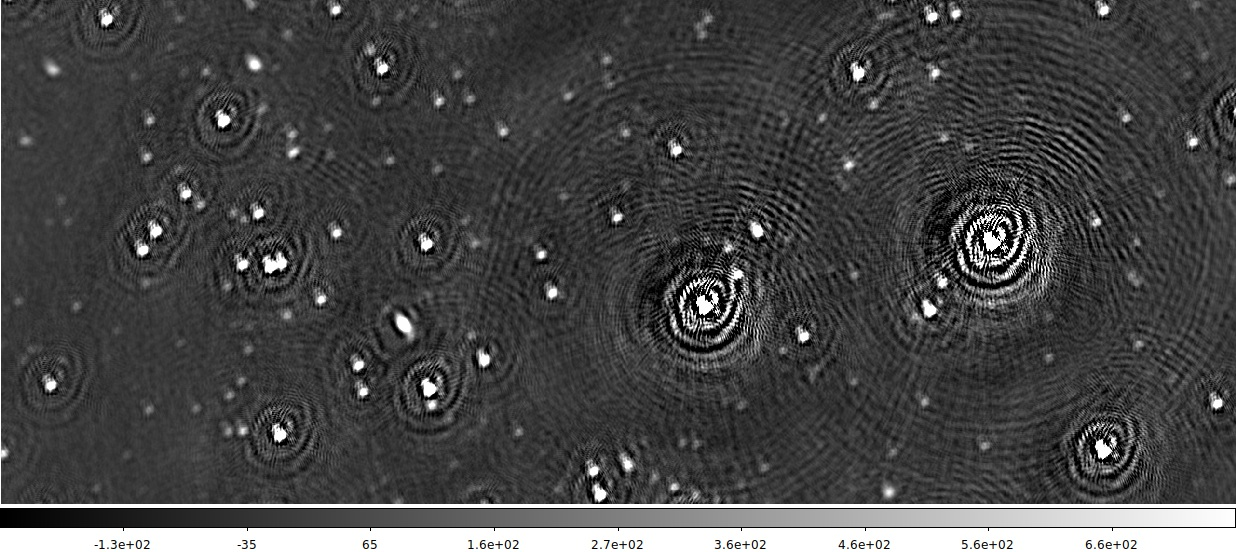
\includegraphics[width=.8\linewidth]{background/figures/raw_image1.jpeg}
    \caption[Image of the raw data]{Raw data for LOFAR observation L229587. We only image half of the bandwidth, from Subband 061 to Subband 183.  }
    \label{fig:L229587_raw}
\end{figure}


\begin{figure}[h]
    \centering
    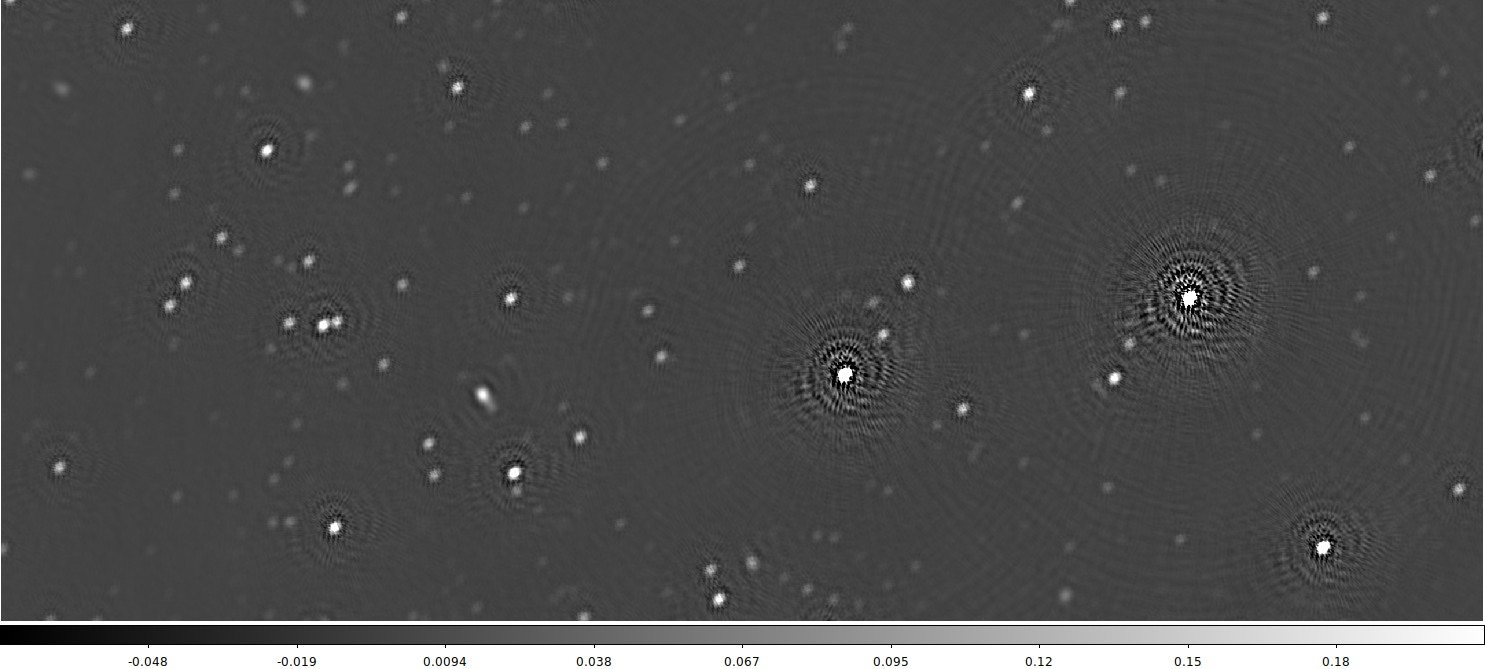
\includegraphics[width=.8\linewidth]{background/figures/prepcal_image.jpeg}
    \caption[Image of preprocessed data]{Preprocessed data for the same observation as figure \ref{fig:L229587_raw}. Note the corrected scale bar, obtained by applying the calibrator solutions.}
    \label{fig:L229587_prepcal}
\end{figure}



\begin{figure}[h]
    \centering
    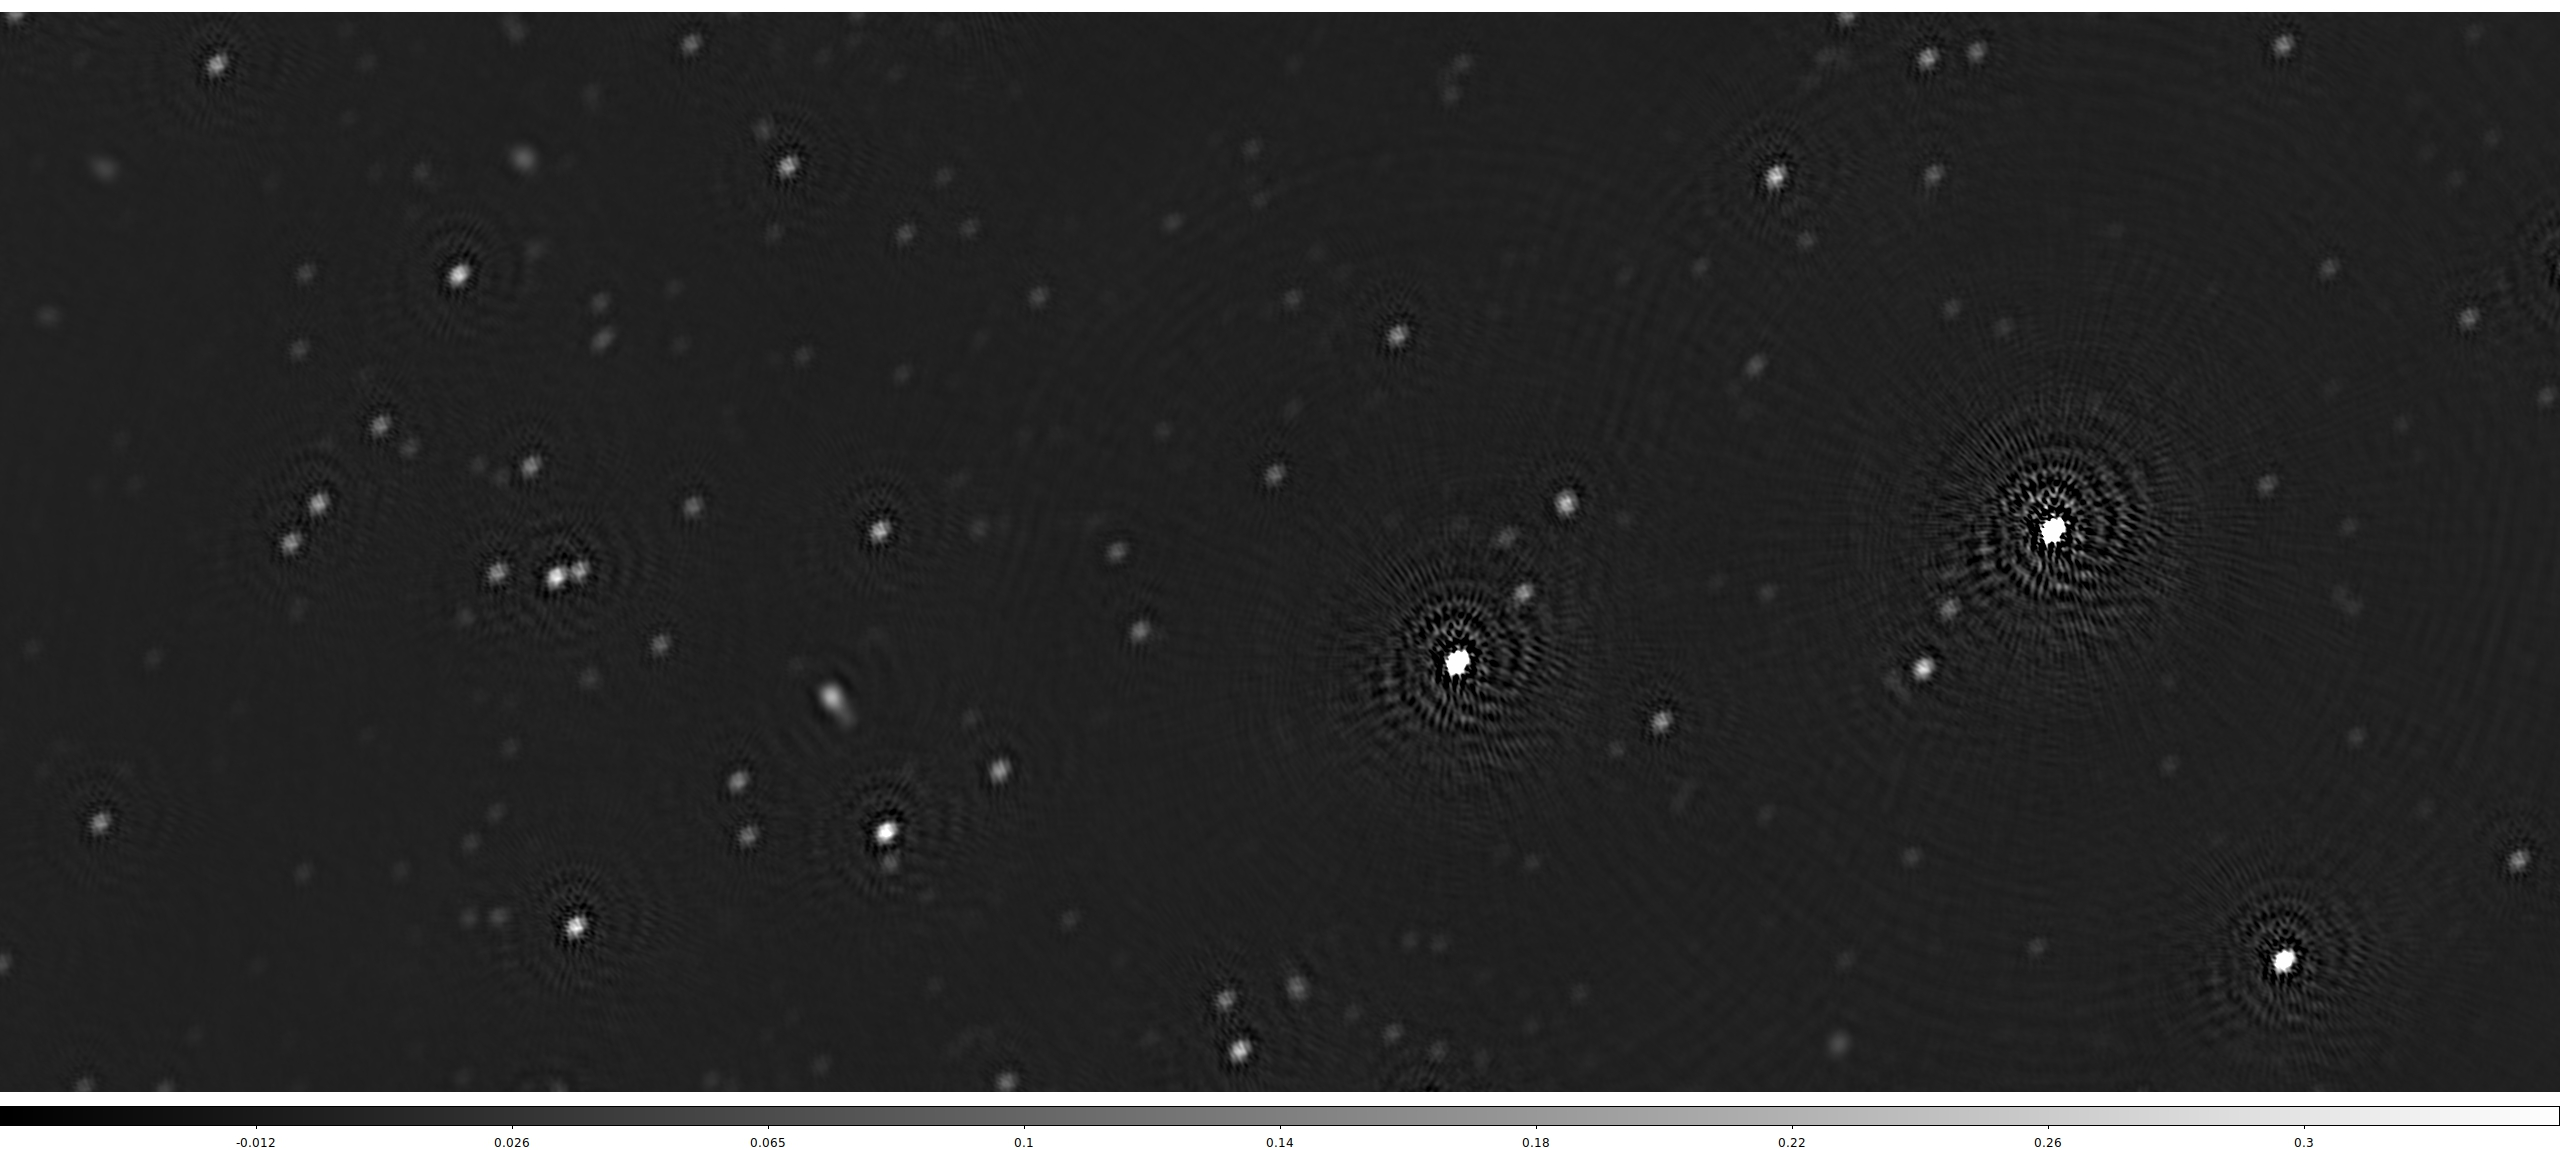
\includegraphics[width=.8\linewidth]{background/figures/INTERP.jpeg}
    \caption[Image of concatenated data]{Data from L229587 after interpolation. }
    \label{fig:L229587_concat_aoflag}
\end{figure}


\begin{figure}[h]
    \centering
    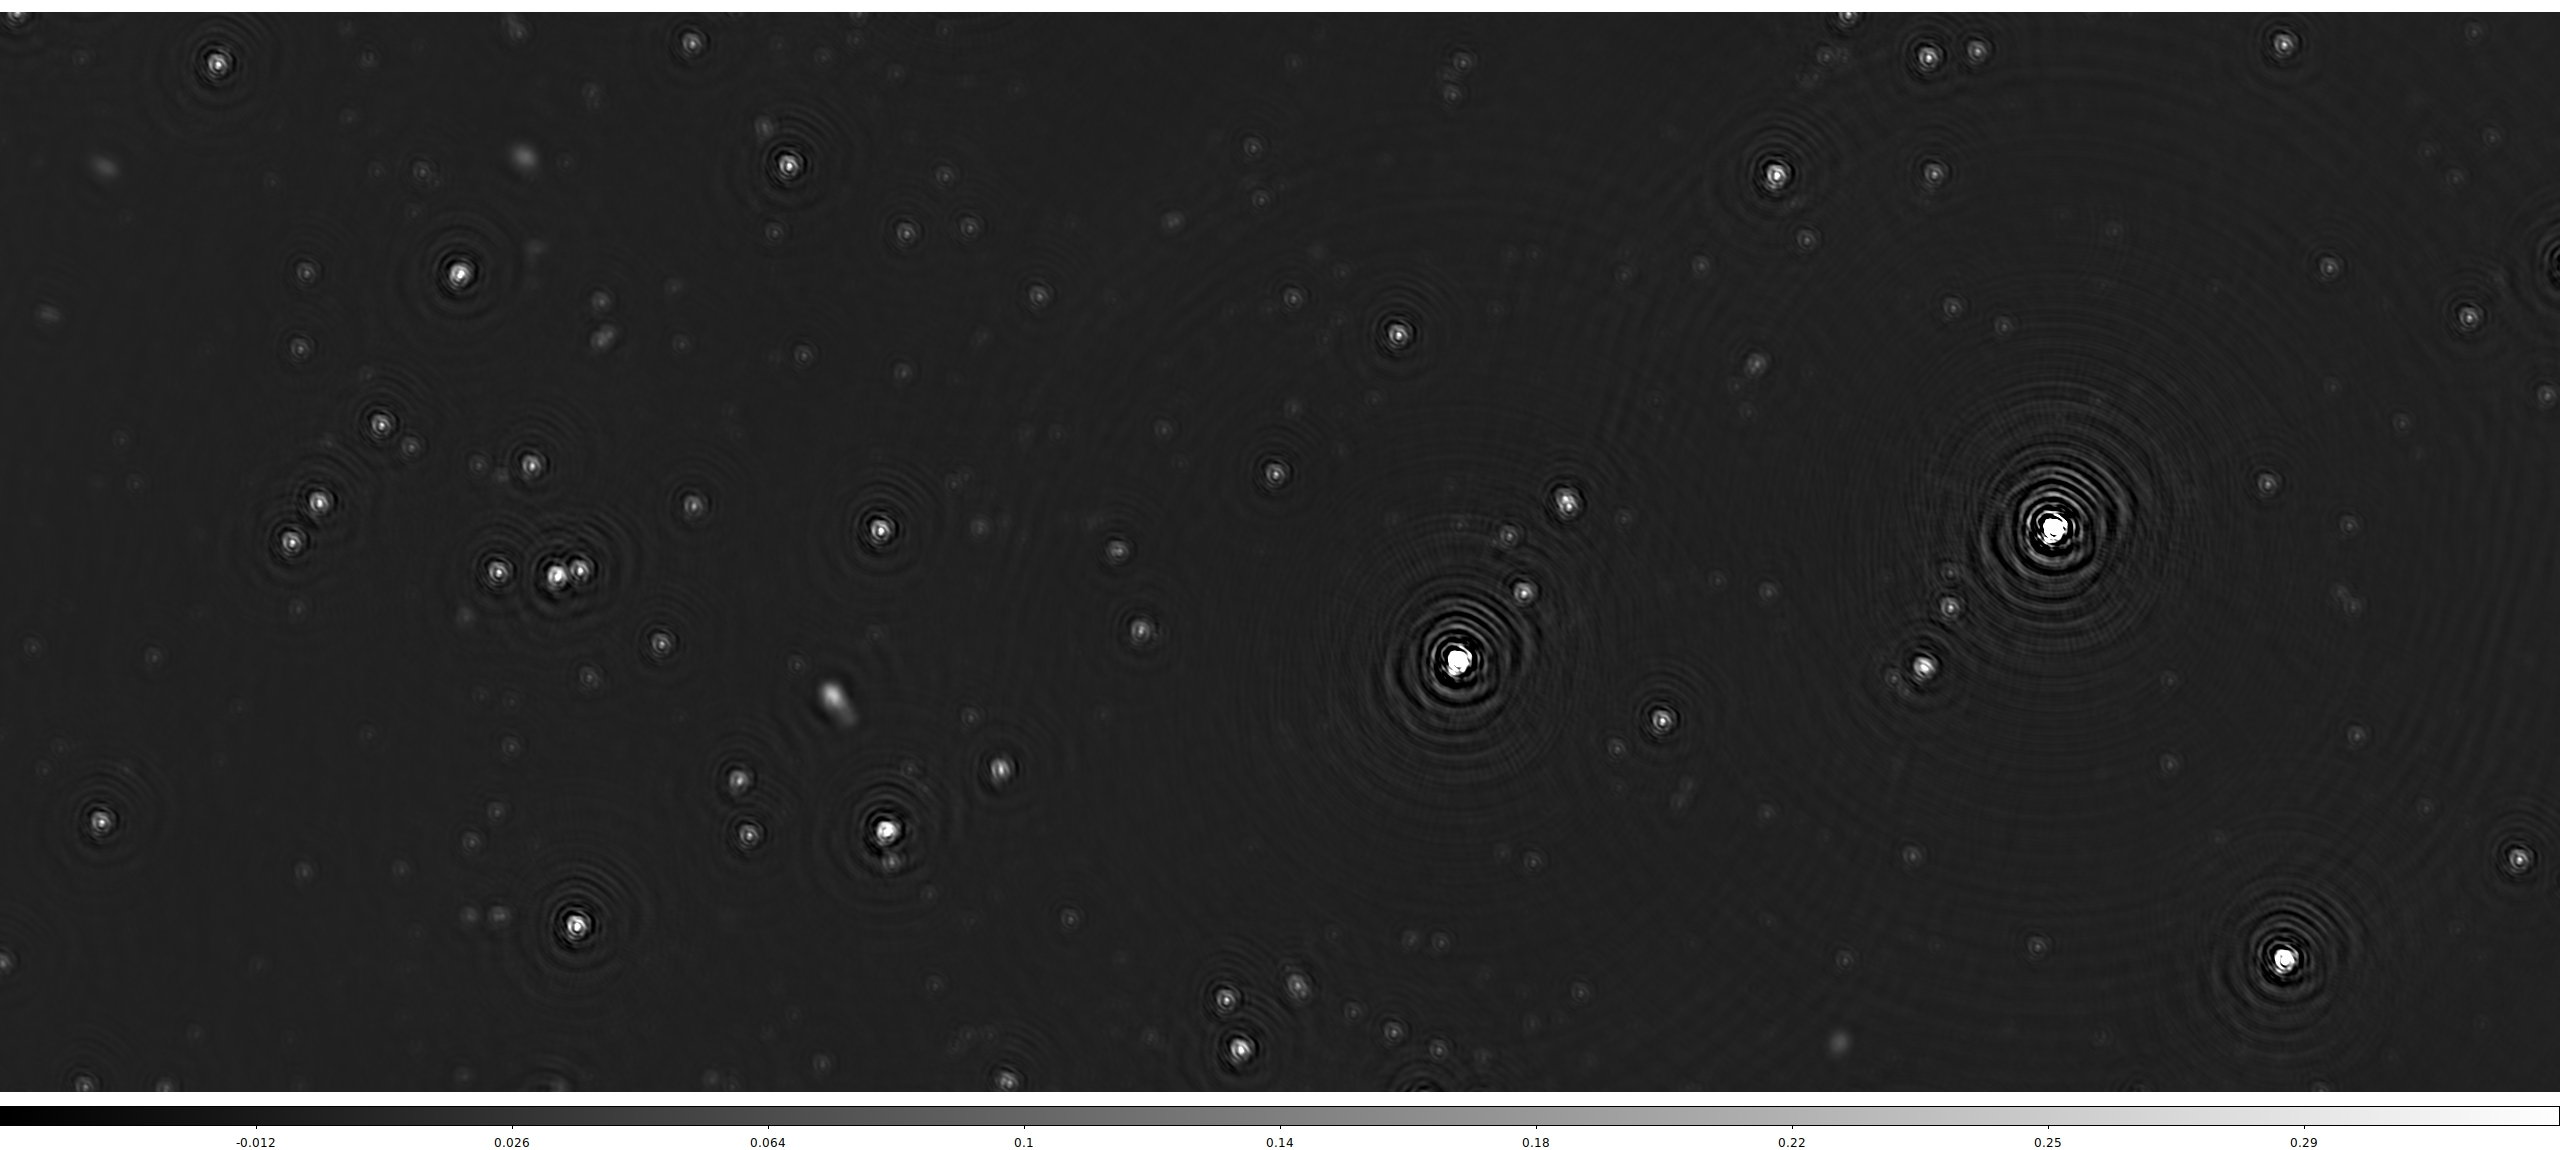
\includegraphics[width=.8\linewidth]{background/figures/final_gsmacl.jpeg}
    \caption[Image of DI calibrated data]{Data from L229587 after calibration against a global skymodel. This calibration removes the direction independent effects}
    \label{fig:L229587_DI_cal}
\end{figure}

\subsection{SURFsara} 

One of the archive locations storing LOFAR data is SURFsara at the Amsterdam Science Park. Aside from a large storage archive, SURFsara also supports several clusters, including the Gina cluster, part of the Dutch Grid infrastructure. Grid computing is a non-interactive application-oriented computational paradigm for distributed computing where a 'grid' consists of a large pool of nodes where users can submit batch jobs. A grid can consist of one cluster or groups of clusters at one or multiple geographical locations, connected with high-speed links and a common job management interface. Using this interface, users can scale out their projects, given that their processing is massively parallel. Computational resources on such a platform are granted based on a scientific proposal and are used freely across the Grid, while jobs are scheduled based on the job requirements and the current resource availability of the grid nodes. This processing paradigm is perfect for large grid-search simulations, but also for the first steps of LOFAR processing. Furthermore, the high-speed connection to the LOFAR archive makes SURFsara a logical location to orchestrate large scale LOFAR projects.


\subsection{LoTSS Processing}

The observations produced by LoTSS will total more than 30 petabytes and require extensive processing before the survey is completed. Each observation is stored as a set of 244 individual files spanning frequency space from 120MHz to 168MHz. Each of these files, named a Subband, is a CASA Measurement set and is identified by its three-digit Subband number, starting from 000. Each Subband, thus, contains a sub-sample of the data in frequency space, stored at a resolution of 1 second and 12.2 kHz per sample. While this high-resolution data is useful for some science cases, our processing algorithms scale with data size, and thus it is necessary to average our data in order to complete the LoTSS processing within the project's time-frame. 

In order to create an image from an archived data set, the data needs to be staged, retrieved and processed. Staging the data refers to sending a request to the archive site to move the data from tape to disk. Once all your data is on disk ('staged'), it is ready to be transferred from the storage to the processing cluster. On this cluster, a science-ready image is produced by processing the raw data through two pipelines. The first pipeline, Direction Independent Calibration pipeline removes artifacts created by `direction independent' effects, i.e. effects that are constant across the field of interest. This pipeline is followed by the Direction Dependent Calibration pipeline which removes effects that change within the field of view.
 
The Direction Independent Calibration pipeline (DI pipeline) consists of two main stages. The first stage is calibration on the calibrator, which uses a short observation of a bright calibration source to determine systematic effects that are independent of the direction of the pointing. The solutions obtained from this step can be applied to the scientific target, improving the data quality. The second step of the DI pipeline is the calibration of the target field against a sky model produced by a previous survey. This calibration determines the gain parameters of all antennas, however it does not correct for effects that vary across the field of view. 
 
In order to create a high fidelity radio image, we need to correct for effects that not only change in time but also across the field of view. These effects, such as the ionosphere or the beam response can be modelled and removed, and their removal is the responsibility of the Direction Dependent pipeline (DD pipeline). Upon successful completion, the DD pipeline produces a radio image that can be used for further scientific studies.

There are a few software packages used to process LOFAR data, typically used in a series of steps creating a processing pipeline. The LOFAR processing pipeline steps use the software, each step encoding the processing parameters in a parameter-set (parset). A pipeline is defined by the list of steps and the parameters of each step concatenated together into a parset file. The LoTSS DI pipeline, \texttt{prefactor} contains a set of scripts used to remove direction independent effects from LOFAR data. Many of the \texttt{prefactor} steps can be executed on the data in parallel: each Subband can be processed independently. Because of the large amount of data, the best architecture for these steps is a cluster of isolated machines with dedicated disks and a high-speed connection to the data. The Dutch grid infrastructure at SURFsara is a logical place to launch these steps. 


\section{Problem Statement and Research Questions}

Radio Astronomy data sets are too large to process in bulk on individual workstations and often strain the resources of small clusters at universities and other institutions. This limitation in resources requires high throughput processing capability, and automation in order to serve processed data in bulk to astronomers. 

\begin{addmargin}[4em]{8em}% 1em left, 2em right
    \emph{\textbf{Problem Statement:} How can we efficiently process broadband LOFAR data in a generic way?} 
\end{addmargin}

The problem statement identifies a very general challenge with LOFAR processing. The LOFAR radio telescope acquires data at a rate of roughly a terabyte per second. This data is stored in a Long Term Archive as it can serve multiple science cases. Our goal is to create the tools for scientists to be able to efficiently process this data with their scripts and software. As such, the tools we build need to be both scalable and generic.   


\subsection{Research Question 1}

To efficiently process LOFAR data, we need to take advantage of the data level parallelism of the early processing steps, each of which can be parallelized by a factor of 244. We investigate a framework for  massively distributed shared platform for this purpose. This leads to our first research question:

\begin{addmargin}[4em]{8em}% 1em left, 2em right
    \emph{\textbf{Research Question 1:} Is it possible to use a distributed shared infrastructure for efficient LOFAR data processing?}
\end{addmargin}

We describe the platform for this processing in Chapters \ref{ch:LOFAR_DSP} and \ref{ch:GRID_LRT}.

\subsection{Research Question 2}

Once we have determined the utility of distributed processing for the LOFAR case, we ask whether a framework can be built to automate large complex workflows. The LOFAR radio telescope serves multiple science cases, each of which is served by a multi-step pipeline with a wide set of parameters. Running an entire pipeline on a single computational node is inefficient, thus the framework developed in Chapters \ref{ch:LOFAR_DSP} and \ref{ch:GRID_LRT} needs to be used to parallelize the relevant steps. This research question asks how to build software to efficiently integrate software pipelines with the distributed platform described previously. 

\begin{addmargin}[4em]{8em}% 1em left, 2em right
    \emph{\textbf{Research Question 2:} How can we build software to easily accelerate complex pipelines for Radio Astronomy?} 
\end{addmargin}

The results of this research question are detailed in Chapters \ref{ch:AGLOW} and \ref{ch:AGOW_CI}, where we detail the software used to automate large scale LOFAR processing as well as a unique use of this software in the LOFAR \texttt{prefactor} Continuous Integration pipeline.  

\subsection{Research Question 3}


How do we collect and process performance statistics per pipeline step and use them to better understand the performance of our software?

Can we create a user portal to make serving LOFAR data easy and efficiently to scientists?






